%%
%%	Initial Management Report
%%	Created by Group02
%%
%%	12:07pm 25/05/2013 
%%
%%	Use for SENG3011
%%

\documentclass[a4paper]{article}
\usepackage{a4wide}
\usepackage[normalem]{ulem} 
\usepackage{graphicx}
\usepackage{lscape}
\usepackage{float}

\begin{document}

%%%%%%%%%%%%%%%%%%%%%%%%%%%%%%%%%%%%%%%%%%%%%%%%%%%%%%%
%%TITLE PAGE
\thispagestyle{empty}
\begin {center}
\Large\textbf{SENG3011} 

\Large\textbf{Intial Management Report}

\bigskip\Large\textbf{Group Number: 02}

\end{center}

\vspace*{16.5cm}
\begin{tabular}{|l|l|}
  \hline
  Version         & 1.7\\\hline
  Print Date      & 19/03/2013 10:26\\\hline
  Release Date    & 27/03/2013\\\hline
  Release State   & Final \\\hline
  Approval State  & Pending \\\hline
  Approved by     & Group02 \\\hline
  Prepared by     & Group02 \\\hline
  Reviewed by     & Group02 \\\hline
  Confidentiality Category  & Confidential\\\hline
\end{tabular}
\pagebreak

%%%%%%%%%%%%%%%%%%%%%%%%%%%%%%%%%%%%%%%%%%%%%%%%%%%%%%%

%%%%%%%%%%%%%%%%%%%%%%%%%%%%%%%%%%%%%%%%%%%%%%%%%%%%%%%
%%REVISION CONTROL

\thispagestyle{plain}     % Turn on page numbering
\setcounter{page}{1}      % set page number counter
\renewcommand{\thepage}{\roman{page}}  % set page number to roman

\noindent{\Large\textbf{Document Revision Control}}\\[2ex]
\begin{tabular}{|l|l|l|l|}
  \hline
  Version & Date & Authors & Summary of Changes\\\hline\hline
	v1.0 & 25/05/2013 & Group02 & Added in Introduction           	\\\hline
	v1.1 & 25/05/2013 & Group02 & Added in Sections 		\\\hline
	v1.2 & 25/05/2013 & Group02 & Added in Requirements table  		\\\hline
	v1.3 & 25/05/2013 & Group02 & Added in Project Management		\\\hline
	v1.4 & 26/05/2013 & Group02 & Added in Architectural MVC 		\\\hline
	v1.5 & 26/05/2013 & Group02 & Added in Use Cases		\\\hline
	v1.6 & 26/05/2013 & Group02 & Added in Architectural Model		\\\hline
	v1.7 & 27/05/2013 & Group02 & Added in Updated Testing Documentation 		\\\hline
	v2.1 & 28/05/2013 & Group02 & Added Code Organisation 		\\\hline

\end{tabular}

\pagebreak

%%%%%%%%%%%%%%%%%%%%%%%%%%%%%%%%%%%%%%%%%%%%%%%%%%%%%%%

%%%%%%%%%%%%%%%%%%%%%%%%%%%%%%%%%%%%%%%%%%%%%%%%%%%%%%%
%%TABLE OF CONTENTS

\tableofcontents
\pagebreak
\listoffigures     %% delete if not required
\pagebreak         %% delete if there is no list of figures

%%%%%%%%%%%%%%%%%%%%%%%%%%%%%%%%%%%%%%%%%%%%%%%%%%%%%%%

%%%%%%%%%%%%%%%%%%%%%%%%%%%%%%%%%%%%%%%%%%%%%%%%%%%%%%%
%%MAIN

\setcounter{page}{1}     % Set page number counter
\renewcommand{\thepage}{\arabic{page}}  % print page number as arabic

\section {Introduction} 

This report is written to discuss our final completed project in terms of the Requirements, Project 
Management and a our own opinion of the project. \\  \\
We also discuss our final design and testing of the system. Where we show you how we took 
our Initial Report and then developed into our final system. Our testing document will be 
provided in this document. We will also provide details how we distributed the workload. 

\newpage

\section {Part 1: Final Management Report} 
\subsection {The Updated Requirement Analysis}

\noindent{\bf Requirements Table}:  \\
    \begin{tabular}{ | l | p{8cm} | p{5cm} |}
    \hline
    {\bf ID} & {\bf Function Requirement} & {\bf Comment} \\
    \hline
    1 & Reading a correctly formatted SIRCA order file (1 day only) & It has been implemented \\
    \hline
    2 & Choosing an appropriate algorithmic trading strategy and setting its different parameters & It has been implemented \\
    \hline
    3 & Generating algorithmic orders for 1 particular day & It has been implemented \\
    \hline
    4 & Generating algorithmic trades for 1 particular day & It has been implemented \\
    \hline
    5 & Evaluating algorithmic trades and providing feedback to user & It has been implemented \\ 
    \hline
    6 & Generating a strategy performance report & It has been implemented \\ 
    \hline 
    7 & GUI functions to control use cases (1-6) to load and execute an orders file & It has been implemented \\ 
    \hline
    8 & GUI functions to visualise market data (spread, volume and depth) & It has been implemented \\ 
    \hline
    \end{tabular} 

\subsection {The Updated Project Management Information} 
\subsubsection {Division of Work}
\indent\indent At the beginning of the project, everyone was given the role of a developer alongside another 
job like team lead, LaTeX expert, tester and quality assurance. After our first report review, 
we modified our roles so that not everyone was a developer, we had Sohaib covering 
requirements and testing, Shanku stayed in a quality assurance role but instead of 
developing as much code as he did before, he was in charge of code sanity and reviewing, 
Michael remained as the document and report generator, retaining his developer role and 
Albert stayed as the team lead and developer.

\subsubsection {Responsibilities and Organisation of the Team}
For each deliverable, Sohaib would provide a detailed explanation and interpretation of the 
requirements to the team so we knew what was expected of us by the delivery date. Following 
the briefing, Albert would decide how the tasks will be tackled and who would be doing which 
parts. Everyone contributed to the information that went into any reports which were 
required with each delivery and our report generator, Michael, would polish and publish the document 
ready for delivery. After development was complete our tester, Sohaib, would begin writing unit
tests and checking if the logic and behaviour complied with the requirements as he interpreted 
them. While this was happening, our quality assurance, Shanku, ran the program several times, 
ensuring that our program provided descriptive outputs and held a quality standard in terms of 
user experience.

Essentially all members of our team had their distinct roles and therefore tasks for each \\
deliverable. There were some dependencies between our team members as we had a structured 
workflow. 

\subsection {Conclusion/Appraisal of Work} 
\indent\indent Overall we believe our project was done well with a couple hiccups along the way. Initially we 
were reluctant to pick at the client for more details about the requirements and designed a system 
which was not what the client was looking for. Another problem we encountered along the 
way was a lack of preparation for our week 10 demonstration. Our group leader was unaware that no 
one else knew how to deploy/export the project into a runnable format, resulting in an inability 
to demonstrate our progress.

Putting the bad aside, the rest of our project was good. All group members contributed equally 
to the project, completing all work on time whenever it was delegated. The end result is a cohesive 
and functional product which adheres to the client�s needs.

\subsubsection {Changes if done differently?}
If we were to do this project again there would be a couple changes. Firstly, we would know 
well ahead of time that we cannot trust the specification by itself and must attempt to gain 
clarification as soon as possible. Should there be any doubts, it would be our job and not the 
client�s job, to clarify the requirements well before initial planning and modelling. Something we 
could have changed was the big picture planning of our project. As a group we did not pay much 
attention to the overall road map of delivery dates along the semester. We feel that it could have 
been beneficial to be more prepared for each delivery date rather than have them creep up on us, 
resulting in a lack of preparation, as seen in our first demonstration.

\newpage

\section {Part 2: Final Design and Testing Report} 
\subsection {The Updated Design}
\subsubsection {Use Cases}

\indent\indent Initially due to some confusion our Requirements weren't what the client specified. We realised
this after handing in the Initial Management Report and after receiving feedback from the client
we were able to correct our initial mistakes and create the following Use Cases:  \\


\noindent{\bf Use Case 1}: Reading Correctly Formatted Sirca File \\
    \begin{tabular}{ | l | p{10cm} |}
    \hline
    	{\bf Actors} & User \\\hline
	{\bf Triggers} & The user starts the program. \\\hline
	{\bf Preconditions} & The user has a correctly formatted Sirca file. \\\hline
	{\bf Postconditions} & The system will be populated with orders \\\hline
	{\bf Normal Flow} & The system starts up, reads in the CSV file and\\
	& prepares the order book of trades.\\\hline
    \end{tabular} \\\\

\noindent {\bf Use Case 2}: Choosing an Algorithmic Trading Strategy \\ 
\begin{tabular}{ | l | p{10cm} |}\hline
	{\bf Actors} & User \\\hline
	{\bf Triggers} & User decides on a trade strategy to try.\\\hline
	{\bf Preconditions} & User has a decided quantity and strategy to trade with. \\\hline
	{\bf Postconditions} & System generates new orders based on specified quantity. \\\hline
	{\bf Normal Flow} & User indicates trading strategy, \\
	& system accepts trade strategy, generates the appropriate \\
	& bids and ask orders and sends it to the trade engine. \\\hline
\end{tabular} \\\\

\noindent {\bf Use Case 3}: Generating Trades for the Day \\ 
\begin{tabular}{ | l | p{10cm} |}\hline
	{\bf Actors} & User \\\hline
	{\bf Triggers} & User has chosen trading strategy and sent it to engine. \\\hline
	{\bf Preconditions} & Algorithmic trades are ready to process and a set of \\
	& orders have already been read in. \\\hline
	{\bf Postconditions} & All algorithmic trades are executed and ready for evaluation. \\\hline
	{\bf Normal Flow} & User tells system to continue with selected trades. \\
	& System executes the algorithmic trades and prepares for evaluation. \\\hline
\end{tabular} \\\\

\newpage
\noindent {\bf Use Case 4}: Evaluating Algorithmic Trades \\ 
\begin{tabular}{ | l | p{10cm} |}\hline
	{\bf Actors} & User \\\hline
	{\bf Triggers} & User wishes to determine the effectiveness of the strategy \\\hline
	{\bf Preconditions} & Algorithmic trades have been processed. \\\hline
	{\bf Postconditions} & The user is given feedback based on the algorithmic trades. \\\hline
	{\bf Normal Flow} & User asks for an evaluation, system finds the percentage gained or lost. \\\hline
\end{tabular} \\\\

\noindent {\bf Use Case 5}: Generating Strategy Performance Report \\ 
\begin{tabular}{ | l | p{10cm} |}\hline
	{\bf Actors} & User \\\hline
	{\bf Triggers} & User wants to see a performance report \\\hline
	{\bf Preconditions} & A strategy has been executed. \\\hline
	{\bf Postconditions} & A report will be generated for the user. \\\hline
	{\bf Normal Flow} & User asks system to generate strategy performance report. \\
	& System provides a performance report to the user.\\\hline
\end{tabular} \\\\

We believe our Use Cases addresses the problem which was presented to us. We were able to
identify which were the main parts of the problem and break them down to 5 uses cases.

\subsubsection {Architectural Diagram}
\indent\indent We had an Architectural Diagram which we first designed and presented in our Initial 
Management Report. After submission and an instructive meeting with the client we were able to correct our
mistakes and finalise an Architectural Diagram where we and the client we satisfied with.  \\ \\

\indent  The final model contains two diagrams, the first which illustrates the communication between 
Users and the System using a Model View Controller diagram.  \\

\indent This Architecture (MVC) has 3 main parts the view, controller and model. The view is what 
the user sees and interacts with, the GUI and Console UI are both located in the view. The view 
commands the controller to carry out task. The controller does functional calls in the model.

\begin {landscape}
\begin{figure}[H]
  \centering
    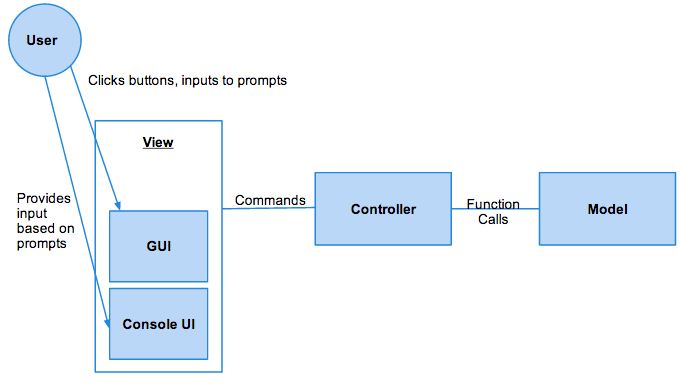
\includegraphics[width=1.4\textwidth]{images/aMVC}
     \caption{Architectural MVC.}
\end{figure}
\end {landscape}

The second which is the Architectural Model illustrating the communication between the 
Trade Signal Generator, Trade Engine and Trade Strategy Evaluator. \\

The Architecture (Model) has 3 main parts the trade signal generator, trade engine and trade 
strategy evaluator. The trade signal generator sends generated signals to the trade engine. The 
trade signal sends matched algorithm trades to the trade strategy evaluator for evaluation. 

\begin {landscape}
\begin{figure}[H]
  \centering
    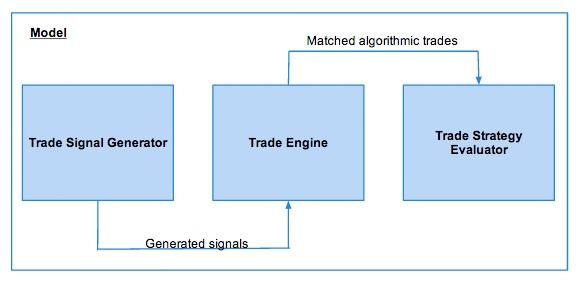
\includegraphics[width=1.3\textwidth]{images/aModel}
     \caption{Architectural Diagram.}
\end{figure}
\end {landscape}

\subsection {The Updated Testing Documentation}
\subsubsection {Initial Feedback}
\indent\indent In our initial feedback we were told even though our test worked it was too vague. As we 
only used one .jar test file it was hard for other users to see what was occurring in our testing. 
Also as we provided no expected output it was even harder for the user to identify if tests worked 
properly. Our test�s were built using JUnit test was in turn ran by the .jar file.This resulted us 
understanding that everything was tested in .jar file while the user had no idea what was being 
tested. 

This resulted in us developing multiple jars so it was easier for others to understand what was 
being tested each time they ran a certain jar file. This was based on the feedback we received for 
the week 10 deliverable.

\subsubsection {New Tests}
\indent\indent We developed new tests for trade matching in the trade engine. Allowing us to check if the
trades matched properly such as price matched. We also further done extensive testing by expanding the 
original tests. We also now have multiple test jar files instead of one big one.

\subsection {Code Organisation} 
\subsubsection {How did our group share the code}
Our group leader set up a git repository which was used to share the code. Git was chosen because 
it is a powerful, distributed version control system that allows multiple users to work on the same 
source files and keep track of the changes. Another great advantage is that git is free to use. Each 
member had their own account which had permissions to push changes to the repository.

\subsubsection {Extra Tools}
Code management was done primarily through git, as mentioned above. Communication and 
delegation of tasks was done via email, phone/sms and Facebook group. Google Docs was mainly 
used to collaborate information as a group and create presentations together at the same time. We 
did not use any dedicated project management tools as we found that our previously established 
communication channels were already very effective.















\end {document}